\documentclass[../../Main/Appunti Fisica.tex]{subfiles}
\begin{document}
Si consideri la figura di seguito riportata.
\begin{figure}[!h]
    \centering
    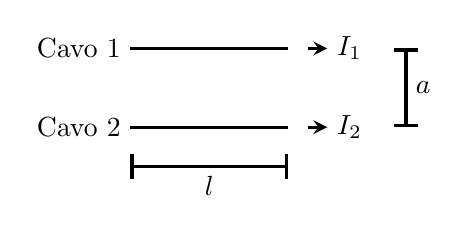
\begin{tikzpicture}[scale = 1, every node/.style={scale=1}]

        % Cable 1
        \node [anchor = east] at (0, 0) {Cavo 1};
        \draw [very thick] (0, 0) -- (2, 0);

        %% Current I1
        \draw [-stealth, very thick] (2.25, 0) -- (2.5, 0);
        \node (I1) [anchor = west] at (2.5, 0) {\(I_{1}\)};

        % Cable 2
        \node [anchor = east] at (0, -1) {Cavo 2};
        \draw [very thick] (0, -1) -- (2, -1);

        %% Current I2
        \draw [-stealth, very thick] (2.25, -1) -- (2.5, -1);
        \node (I1) [anchor = west] at (2.5, -1) {\(I_{2}\)};

        \draw [|-|, very thick] (0, -1.5) -- (2, -1.5);
        \node [anchor = north] at (1, -1.5) {\(l\)};

        \draw [|-|, very thick] (3.5, 0) -- (3.5, -1);
        \node [anchor = west] at (3.5, -0.5) {\(a\)};

    \end{tikzpicture}
    \caption{Cavi percorsi da corrente, posti a distanza \textit{a} di lunghezza \textit{l}.}
    \label{fig:17}
\end{figure}

Calcolando la forza \(\vb{F_{1}}\) esercitata sul cavo 2 dal cavo 1, poiché il cavo 2 produce un campo \(\vb{B_{2}}\) nella regione di spazio del cavo 1, segue
\[
    \vb{F_{1}} = I_{1} l \vb{B_{2}} = Il\left( \frac{\mu_{0} I_{2}}{2 \pi a} \right) = \frac{\mu_{0} I_{1} I_{2}}{2 \pi a} l
\]
analogamente si trova \(F_{2}\), dal cui calcolo si trova che le due sono uguali in modulo e direzione, ma opposte in verso.
\end{document}
\clearpage